% ILLIXRLink{path} links to path at a fixed commit.
\newcommand{\ILLIXRlink}[1]{\href{https://github.com/ILLIXR/ILLIXR/tree/6c25003f79ecc35b4e002615b5a05d3077851d90}{\texttt{#1}}}

\section{Implementation}

\footnote{Our implementation is located at: \href{https://github.com/ILLIXR/ILLIXR/tree/illixr-testing}{\texttt{https://github.com/ILLIXR/ILLIXR/tree/illixr-testing}}}

\subsection{R.Q. 1 Approximation Testing}

With the following infrastructure, we can test out different approximations and manually inspect the output for acceptance for \textbf{R.Q. 1}.
We also need to know how much time the approximation saves, so we know if it is `worth it.'
The data we collected on compute-times are shown in \cref{compute-times}.

\begin{figure}
  \label{compute-times}
  \caption{Compute times for various approximation configurations (lower is better).}
  \todo{Insert graph}
\end{figure}

\subsubsection{Approximation Knobs}

ILLIXR uses state-of-the-art components such as OpenVINS \cite{Geneva2020ICRA} for SLAM.
We located approximation knobs in OpenVINS and consulted domain experts on which ones should be modified and tuned.\footnote{
  \todo{href to https://github.com/ILLIXR/open\_vins/blob/illixr-testing/ov\_msckf/src/slam2.cpp\#L30}
}

\begin{table*}
  \centering
  {
    \caption{OpenVINS approximation knobs. See OpenVINS documentation for more details\cite{Geneva2020ICRA}.}
    \begin{tabularx}{\linewidth}{r||l|X}
      \textbf{Knob} & \textbf{Range} & \textbf{Meaning} \\
      & {(approx. first)} & \\
      \hline\hline
      \verb+num_pts+ & 50--300 & The number of points extracted and tracked in each image frame \\
      \verb+use_rk4_integration+ & [false, true] & If Rk4 imu integration is used\\
      \verb+use_stereo+ & [false, true] & Whether cameras are stereo or binocular. If binocular, it does monocular feature tracking on each image \\
      \verb+use_klt+ & [false, true] & Uses KLT tracking or descriptor matcher \\
      \verb+downsample_camera+ & [true, false] & Halves the resolution all tracking image \\
      \verb+enable_async_reproject+ & [false, true] & (outside of OpenVINS, elsewhere in ILLIXR) queries a current pose and reprojects the frame just before display, making up for some latency in SLAM \\
    \end{tabularx}
  }
\end{table*}

The exact set of knobs is not so significant, as long as I have some useful ones, some useless ones, and they are orthogonal.

\subsubsection{Timing Infrastructure}

In order to test the approximations, I need to know how much time they are saving. Timing ILLIXR is not straightforward.
\begin{itemize}
\item Whole-program CPU time won't work because, because ILLIXR will find another way to spend the spare cycles.
\item \verb+perf+ won't work because it does not have dynamic information (the arguments) of the function. It is thus impossible to disambiguate which component to charge a function-call to.
\item Language-level tools won't work because they are oblivious to threads launched and joined inside a function. Several functions in OpenVINS launch a short-running thread to parallelize the computation.
\end{itemize}

Since none of these off-the-shelf solutions will work, we created a lightweight framework for CPU time logging.
At each function one wants to instrument, one can call a macro with a static label (such as a function name) and dynamic label (such as arguments that disambiguate the function-call).
We use \verb+clock_gettime+ to measure the actual time the thread spends scheduled.
We use resource-acquisition-in-initialization RAII to automatically time the enclosing scope.
Creating the RAII object pushes the current call onto a thread-local stack.
These stack-frame times get pushed onto a global list and serialized only at the very end of the program, so as to not perturb performance during execution\footnote{\todo{href to common/cpu\_timer3.hpp}}.

\subsection{R.Q. 2 Automatic Approximation Testing}

In order to automatically accept or reject approximations, we collect system-level error metrics.
The data we collect is shown in \cref{errors}.
In a real system, we would determine a threshold of acceptability from user-studies, but that is outside the scope of this project;
  we will continue under the assumption that \textit{there is some} threshold.

\begin{figure}
  \label{errors}
  \caption{System-level error for various approximation configurations (lower is better).}
  \todo{Insert graph}
\end{figure}

\subsubsection{Approximation Configuration Infrastructure}

We created a script that runs ILLIXR over an arbitrary set of approximation configurations.
The script configures ILLIXR by generating an ILLIXR configuration file and environment variables.\footnote{\todo{href to experiment.py:run\_illixr}}

\subsubsection{System-Level Metrics}

In the interest of repeatability, we switched to ILLIXR's offline-mode which uses a dataset on disk instead live sensor data.
We used the EuRoC dataset, which has high-quality ground-truth pose data \cite{Burri25012016}.

The output of an XR system with pre-recorded sensor trace is essentially a video stream.
Capturing the video-stream is non-trivial because dumping frames eagerly would perturb the computation, while deferring until the end of the computation involves buffering which has proven too memory intensive.
Since ILLIXR uses OpenGL commands to draw frames, we can just capture every OpenGL command in a binary format and replay those commands offline.
This is exactly what the \verb+apitrace+ tool does \cite{apitrace}.\footnote{\todo{href to experiment.py:159}}

We generate that video-stream from the ground-truth data, and then compare the two frame-by-frame.
First, we tried using Structural Similarity Index Metric (SSIM), which has been used to compare XR video streams before \todo{citation}\footnote{\todo{href video\_dist.py:compute\_ssim}}.
However, this may not be the best metric to compare video streams which have variation in their pose.

With SSIM performing poorly, we also tried a hand-made metric we call \ul{homography-distance}:
For each frame of the both videos, we use SIFT to identify comon features in both frames \todo{cite SIFT} and take the mean difference in position (we also tried median and max difference).\footnote{\todo{link to video\_dist.py:compute\_feature\_dist}}
Like a user, it emphasizes rotations (in which every pixel moves) over translations (in which only pixels on foreground objects move).
Most of the inaccuracies in homography-distance correspond to valid relaxations of user acceptance.
For example, SIFT will be unable to detect many features if the background is uniform (say your looking at a blue sky),
    but a human user, unable to lock onto any feature, would also be less able to detect small movements and would be more forgiving.

\subsection{R.Q. 3 Fast Automatic Approx Testing}

The prior method involves running the whole system for one minute (enough time to collect a representative trace), about two minutes to replay the OpenGL trace, and ten minutes to compute the video distances.
Ideally, we could use approximation auto-tuning such as ApproxHPVM \cite{approxhpvm}, but this goal is still quite far away. First, we need to evaluate system-level effects of approximations at a much faster rate.

\subsubsection{Estimating System-Level Error by Component-Level Proxies}

The component-level metrics are much easier to get than the system-level ones.
Only a small set of components have to be run, and they can be run without realtime scheduling (no need to \verb+sleep+ to get the timing right).
Determining the system-level error from the component-level error analytically is too difficult.
AR/VR systems have multiple paths from SLAM to the output, which makes the error \textit{non-compositional}.
For example, errors SLAM at time \(t\) in render can be corrected by SLAM at \(t+\delta\) through the timewarp (in \cref{dag}).

\begin{figure}
\caption{AR/VR DAG, showing how SLAM flows to the output over multiple paths.}
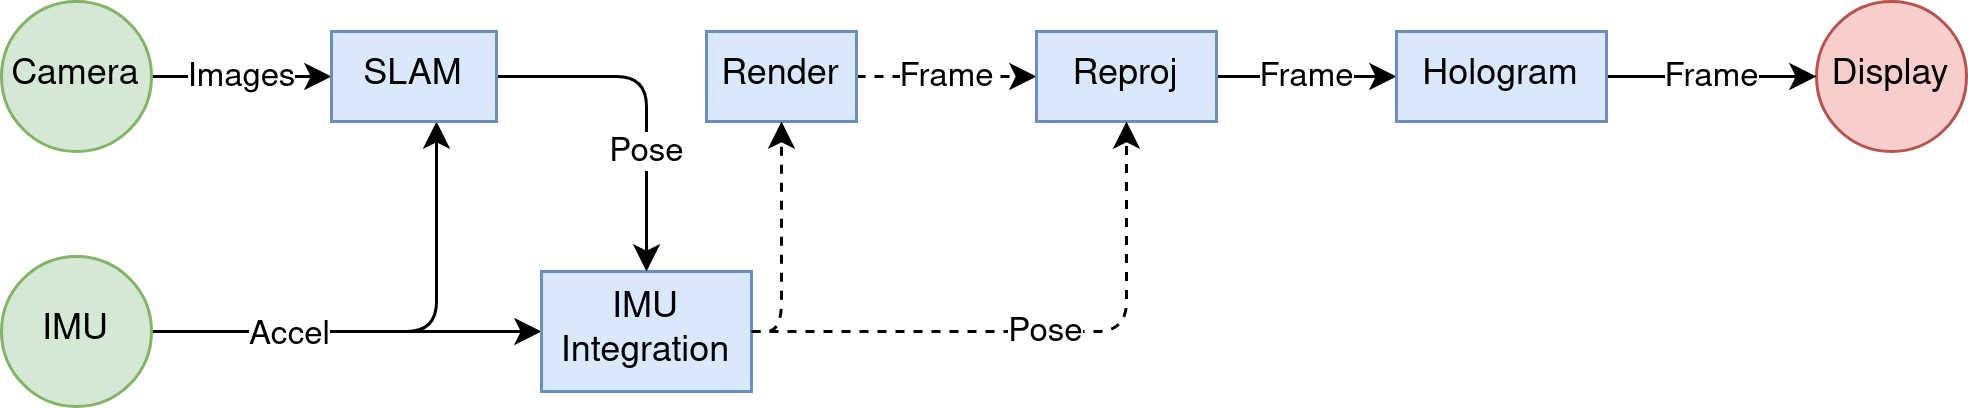
\includegraphics[height=1.8cm]{dag.png}
\label{dag}
\end{figure}

Instead of an analytical model, we might consider an empirical one, using machine learning techniques.
We have both binary-valued knobs and continuous knobs.
It is possible that the effect of each knob is also non-compositional;
turning on two approximations simultaneously could have a different impact than turning them both on separately.
Therefore, a two- or three-layer fully-connected neural network will probably be able to capture \todo{finish writingf}

\subsubsection{Component-Level Metrics}

For SLAM-level metrics, we compare the poses SLAM returned to the ground-truth.
However, since the ground-truth data was collected by different sensors, it is stored in a different frame-of-reference.
We used the Umeyama's Method to register a correspondence from SLAM's poses to the ground-truth dataset for one for a non-approximate SLAM\cite{88573}.
This provided the coordinate transformation we could use for the rest of the approximation-trials.\footnote{This alignment applies to the System-Level video metrics as well; \todo{href to ILLIXR/common/pose\_prediction:gt\_transform}}
This transformation is shown in \cref{transformation}.

\begin{figure}
  \label{transformation}
  \caption{Unaligned and aligned poses, with dotted arrows showing the transformation. It only appears that the transformation `distorts' space because the transformation rotates `out of the plane'. This is a 2d projection of a 3d trajectory, so there is a part of the trajectory you can't see.}
  \todo{Same figure from progress5.md}
\end{figure}

We compute the euclidean distance in position-displacement the angular distance of the orientation-displacement.
These errors have a vastly different impact on users.
Rotations are the most important movement, because even if the user only moves a few degrees, everything in the world moves by an appreciable pixel-distance;
However, with translation, distant objects stay in roughly the same place. Only foreground items respond to head-translations.
Notice that mean-homography-distance implicitly captures this too:
if every object in the scene moves roughly the same amount due to rotation and a few objects in the foreground move due to translation, then the mean distance will be mostly influenced by the background but a little by the foreground too.
The component-level error we collected is also shown in \cref{errors}.
